\documentclass[12pt,oneside]{book}

% Page layout: small margins
\usepackage[margin=2.5cm]{geometry}

% Encoding and font
\usepackage[T1]{fontenc}
\usepackage[utf8]{inputenc}
\usepackage{lmodern}
\usepackage{microtype}

% Math and theorem tools
\usepackage{amsmath,amssymb,amsthm,mathtools}
\usepackage{siunitx}

% Graphics and floats
\usepackage{graphicx}
\usepackage{booktabs}

% References and links
\usepackage[dvipsnames]{xcolor}
\usepackage[colorlinks=true,linkcolor=MidnightBlue,citecolor=OliveGreen,urlcolor=BrickRed]{hyperref}
\usepackage[nameinlink]{cleveref}

% Counters per chapter
\usepackage{chngcntr}
\numberwithin{equation}{chapter}
\counterwithin{figure}{chapter}
\counterwithin{table}{chapter}

% Paragraph spacing (optional)
\setlength{\parindent}{0.0em}
\setlength{\parskip}{1.0em} 

% Metadata
\title{Basics of Newtonian Mechanics}
\author{İskender Yalçınkaya, Ph.D. \\
        \small{Department of Physics} \\
        \small{FNSPE, CTU in Prague}}
\date{\today}

\begin{document}
\frontmatter
\maketitle
\tableofcontents

\mainmatter

\chapter{Mathematical Tools}
\section{Scalars and Vectors}
\section{Rate of Change and Derivatives}
\chapter{Kinematics}
Here we will study the motion of particles over time without considering the causes of the motion.

\section{Particle}

A \emph{particle} is an abstract object with mass but occupies no volume. From the geometrical point of view it is a point with an associated mass. We use this abstraction to describe objects whose dimensions are negligable in describing its motion. For example, the planets may be considered as particles for their motion around the sun. It is worth mentioning that this assumption brings the density of a particle to be infinite by definition, since it occupies no volume.

\section{Position}
To locate a particle in space we need an origin $O$ where we measure distances from. If the particle lives in one-dimensional space, like a bead on a wire, we can use a single real number $x$ to denote its position relative to the origin. If the particle lives in a two-dimensional space, like an ant on a table, we need two real numbers $(x,y)$ to specify its position. Finally, if the particle lives in a three-dimensional space, like a bird flying in the sky, we need three real numbers $(x,y,z)$ to denote its position.

\section{Linear Motion}
Linear motion refers to the movement of a particle along a straight line.

\section{Rotation}

\section{Spiral motion}

\section{Cycloidal motion}



\section{Oscillation}

Oscillations are periodic motions; they repeat themselves after a certain interval of time. Complex numbers together with the exponential function provide a powerful and neat framework for describing and analyzing oscillatory phenomena.

\subsection*{Complex Numbers}

Mathematicians figured in the 16th century that cubic formulas sometimes yield three real solutions while still forcing square roots of negative numbers to appear in the intermediate algebra; rules for $\sqrt{-1}$ were then introduced to keep these calculations consistent and recover the real results, marking the first systematic use of complex numbers. It was Descartes who coined the term ``imaginary'' for these numbers, reflecting the skepticism of the time regarding their existence, then Euler adopted the notation $i$ for $\sqrt{-1}$ making the calculation routine, which has since become standard in mathematics.

Complex numbers are numbers that can be expressed in the form 
\begin{equation}
    z = x + iy
\end{equation}
where $x$ and $y$ are real numbers, and $i$ is the imaginary unit satisfying the equation $i^2 = -1$. We call them ``numbers'' because they can be added, subtracted, multiplied, and divided like real numbers; they follow the same algebraic rules as real numbers, with the additional rule that $i^2 = -1$.

The real part of the complex number is denoted by $\text{Re}(z) = x$, and the imaginary part is denoted by $\text{Im}(z) = y$. Complex numbers can be represented graphically on the complex plane, where the horizontal axis represents the real part and the vertical axis represents the imaginary part as shown in Fig.~\ref{complex-plane.png}. 
\begin{figure}[htbp]
    \centering
    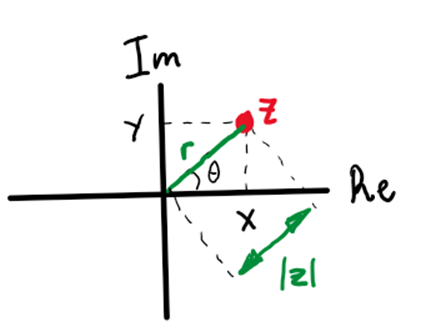
\includegraphics[width=0.4\textwidth]{figures/complex-plane.png}
    \caption{The complex plane}
    \label{complex-plane.png}
\end{figure}

Following the Pythagorean theorem, the magnitude (or modulus) of a complex number $z = x + iy$ is given by
\begin{equation}
    |z| = \sqrt{x^2 + y^2}
\end{equation}
which defines the distance of the point $(x, y)$ from the origin in the complex plane. The argument (or angle) of a complex number is the angle $\theta$ formed with the positive real axis, and it can be calculated using the arctangent function:
\begin{equation}
    \theta = \tan^{-1}\left(\frac{y}{x}\right)
\end{equation}
It is often useful to express complex numbers in polar form:
\begin{equation}
    z = r (\cos \theta + i \sin \theta) 
\end{equation}
where $r = |z|$ is the magnitude and $\theta = \arg(z)$ is the argument of the complex number. When $r$ is kept constant and the angle $\theta$ is changed linearly with time, the complex number $z$ traces out a circle in the complex plane, which can be interpreted as a representation of oscillatory motion. To connect $\theta$ with time, we can set $\theta = \omega t + \phi$, where $\omega$ is the \emph{angular frequency} of the oscillation (in units 1/[T]) and $\phi$ is the phase constant. Thus, we can rewrite the polar form of the complex number as:

\begin{equation}
    z(t) = r \left( \cos(\omega t + \phi) + i \sin(\omega t + \phi) \right)
\end{equation}
\subsection*{The exponential function}
The exponential function $e^x$ is a mathematical function that describes growth or decay processes as shown in Fig.~\ref{fig:exponential-function}. 
\begin{figure}[htbp]
    \centering
    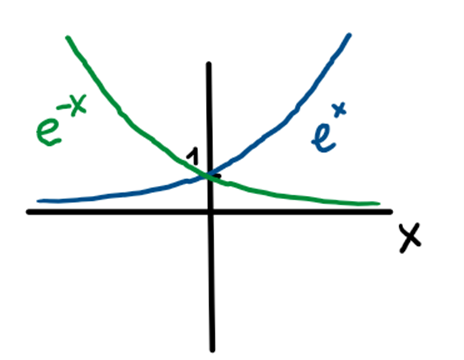
\includegraphics[width=0.4\textwidth]{figures/exponential-function.png}
    \caption{The exponential function $e^x$ showing growth for positive $x$ and decay for negative $x$.}
    \label{fig:exponential-function}
\end{figure}
It is the only function that is equal to its own derivative, meaning that the rate of change of the function at any point is proportional to the value of the function at that point:
\begin{equation}
    \frac{d}{dx} e^x = e^x
\end{equation}
If, for example, the position of a particle changes exponentially with time as $x(t) = e^{t}$, then its velocity is also given by $v(t) = \frac{dx}{dt} = e^{t}$, which is the same as its position function. Hence, if at $t=0$, the particle is at position $x(0) = e^0 = 1$, its velocity at that instant is also $v(0) = e^0 = 1$. At time $t=1$, the position becomes $x(1) = e$, and the velocity is also $v(1) = e$. If we consider another exponential function with a \emph{growth rate} $k$, then the position and velocity functions become $x(t) = e^{kt}$ and $v(t) = \frac{dx}{dt} = k e^{kt}$, respectively. In this case, the velocity is proportional to the position by a factor of $k$:
\begin{equation}
    \frac{d}{dt}\underbrace{e^{kt}}_{\text{position}} = \underbrace{ke^{kt}}_{\text{velocity}}
\end{equation}
If the exponent is a negative number, the function describes exponential decay instead of growth. For instance, if the position of a particle changes as $x(t) = e^{-t}$, its velocity is given by $v(t) = \frac{dx}{dt} = -e^{-t}$, indicating that the particle is slowing down over time. If we consider the initial condition $x(0) = 1$, then the velocity at that instant is $v(0) = -1$. As the particle goes towards the origin, its position decreases exponentially, and its velocity becomes less negative, approaching zero as time progresses.

\subsection*{Complex Exponential Function}
What if we replace the exponent $x$ in the exponential function $e^x$ with a complex number $z = x + iy$? First let us consider a simpler case where the exponent is purely imaginary, i.e., $z = i\theta$ where $\theta$ is a real number. In this case, the complex exponential function can be expressed as:
\begin{equation}
    e^{i\theta} = \cos \theta + i \sin \theta
\end{equation}

The exponential function $e^x$ is often recognized for its unique property that its derivative is equal to itself. It is an analytical function that can be defined through its Taylor series expansion:
\begin{equation}
    e^x = \sum_{n=0}^{\infty} \frac{x^n}{n!} = 1 + \frac{x}{1!} + \frac{x^2}{2!} + \frac{x^3}{3!} + \ldots
\end{equation}

Couldn't we use a cosine or sine function to decribe oscillations instead of complex numbers? The answer is yes, but complex numbers provide a more elegant and efficient way to handle oscillatory phenomena, especially when dealing with multiple oscillations or when performing mathematical operations such as differentiation and integration. Using Euler's formula, we can express the complex exponential function as:
\begin{equation}
    e^{i\theta} = \cos \theta + i \sin \theta
\end{equation}
This relationship allows us to rewrite the polar form of a complex number in terms of the exponential function:
\begin{equation}
    z(t) = r e^{i(\omega t + \phi)}
\end{equation}
This representation is particularly useful in physics and engineering, as it simplifies the analysis of oscillatory systems. For example, when dealing with differential equations that describe oscillatory motion, using complex exponentials can make the calculations more straightforward. Additionally, complex numbers facilitate the representation of phase relationships between different oscillations, which is essential in many applications such as signal processing and wave mechanics.

\chapter{Dynamics}
In principle, we can measure how a given particle accelerates by observing its motion. However, to understand \emph{why} it accelerates, we need to identify the forces acting on it. In this chapter, we will introduce the concept of force and explore Newton's laws of motion, which form the foundation of classical mechanics. We will also discuss various types of forces, such as gravitational, electromagnetic, and contact forces, and how they influence the motion of particles.

\chapter{Small oscillations}
In this chapter, we will study how physical systems behave in the vicinity of their stable equilibrium points. Such behavior is often referred to as \textit{small oscillations} because the system exhibits a oscillatory motion about its equilibrium point and it's displacement is small. We will first start with the description of complex numbers for they are heavily related to oscillatory motion. Then, we will discuss the dynamics of a single particle undergoing small oscillations.
\begin{figure}[htbp]
    \centering
    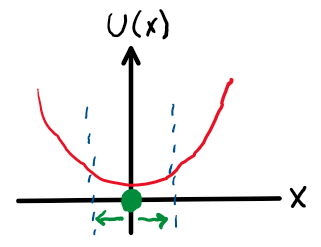
\includegraphics[width=0.38\textwidth]{figures/small-oscillation.png}
    \caption{A particle (green) with a total energy $E$ bouncing back and forth (oscillating) in between points $x_1$ and $x_2$ about its stable equilibrium point at $x_0$ in a potential $U(x)$. The amplitude of oscillation is $A$. The choice of the minimum of the potential as the reference is totally arbitrary.}
    \label{fig:small-oscillations}
\end{figure}



\section{Dynamics of Small Oscillations}
We will study how physical systems behave in the vicinity of their stable equilibrium points. Such behavior is often referred to as \textit{small oscillations} because the system exhibits a oscillatory motion about its equilibrium point and it's displacement is small. We will restrict our attention to one-dimensional systems for simplicity. More specifically, we are interested in the dynamics of a particle whose potential is defined under three assumptions:
\begin{enumerate}
    \item[(i)] $U(x)$ is an analytic function of $x$.
    \item[(ii)] $U(x)$ has a local minimum at $x = x_0$, i.e. $U'(x_0) = 0$ and $U''(x_0) > 0$, which implies that $x_0$ is a stable equilibrium point.
    \item[(iii)] The displacement from equilibrium $|x - x_0|$ is sufficiently small.
\end{enumerate}
Assumption (i) allows us to express the potential as a Taylor series expansion about the equilibrium point $x_0$:
\begin{equation}
    U(x) = U(x_0) + U'(x_0) (x - x_0) + \frac{1}{2} U''(x_0) (x - x_0)^2 + \frac{1}{6} U'''(x_0) (x - x_0)^3 + \ldots 
\end{equation}
Assumption (ii) asserts that the first derivative of the potential vanishes at $x_0$ and that the second derivative is positive. Moreover, assumption (iii) implies that the displacement is deliberately made small enough such that the third and higher-order terms in the Taylor series expansion can be neglected compared to the quadratic term. Together with the fact that the reference level of potential energy can be chosen arbitrarily (i.e., $U(x_0) = 0$), these assumptions lead to a potential given as follows:
\begin{equation}
    U(x) = \frac{1}{2} k (x - x_0)^2
    \label{eq:quadratic-potential}
\end{equation}
where $k \equiv U''(x_0) > 0$. It is worth emphasizing that this form of potential is a direct consequence of the three assumptions stated above, and it is not limited to specific systems like springs or pendulums. In other words, choosing the potential as you see in \eqref{eq:quadratic-potential} is equivalent to writing down the assumptions we stated above. In fact, almost all physical systems can be approximated by this quadratic potential near their stable equilibrium points. This universality is a powerful aspect of the small oscillations framework, as it allows us to analyze a wide range of systems using a common mathematical approach.

\begin{figure}[htbp]
    \centering
    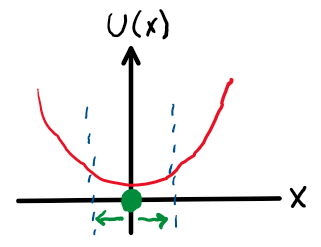
\includegraphics[width=0.4\textwidth]{figures/small-oscillation.png}
    \caption{Small oscillations}
    \label{fig:small-oscillations}
\end{figure}

Given the quadratic potential, one can derive the force acting on the particle as follows:
\begin{equation}
    F(x) = -\frac{dU}{dx} = -k (x - x_0)
\end{equation}
which is known as Hooke's law. It is a \emph{restoring force} that pulls the particle back towards the equilibrium position $x_0$ whenever it is displaced. The dynamics of the particle can be described by Newton's second law:
\begin{equation}
    F_\text{net} = m \ddot{x}
\end{equation}
where $m$ is the mass of the particle. Since the restoring force is the only force acting on the particle, we can substitute it into Newton's second law by setting $x_0=0$ for simplicity and without loss of generality:
\begin{equation}
    m \ddot{x} = -k x
\end{equation}
This is a second-order linear differential equation that describes simple harmonic motion. If we rearrange the equation, we obtain:
\begin{equation}
    \ddot{x} + \omega_0^2 x = 0
\end{equation}
where $\omega_0^2 \equiv \frac{k}{m}$. The reason why we start calling $k/m$ as the square of a new variable $\omega_0$ will become clear soon. For now you can safely think that it is being done to just keep the notation simple.

\appendix
\chapter{Linear Algebra Facts}
If $\mathbf{M}$ is symmetric positive definite, eigenvectors corresponding to distinct eigenvalues are $\mathbf{M}$-orthogonal.

\backmatter
% Uncomment to add references via BibTeX:
% \bibliographystyle{plain}
% \bibliography{references}

\end{document}